\clearpage

\chapter{Implementierung}

\section{Allgemeines}
Die Implementierung wurde für alle Lastenheftfunktionen der Priorität 1 umgesetzt. Alle Elemente der grafischen Benutzeroberfläche sind ohne GUI-Builder erstellt worden. Der Programmcode liegt als .java Dateien vor und kann über den Aufruf von Main.java ausgeführt werden.

\section{Umfang}
Es wurden 16 Klassen mit insgesamt 1281 Lines of Code implementiert.

\begin{figure}[!h]
	\centering
    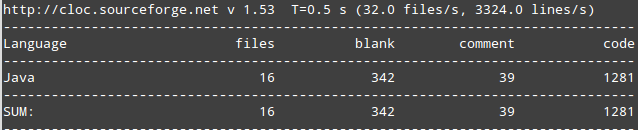
\includegraphics[width=\textwidth]{./cloc.png}
	\label{layout_gesamt}
\end{figure}


%GUI
\clearpage
\section{Benutzerobefläche}

\subsection{Hauptmenue}
\begin{figure}[!h]
	\centering
    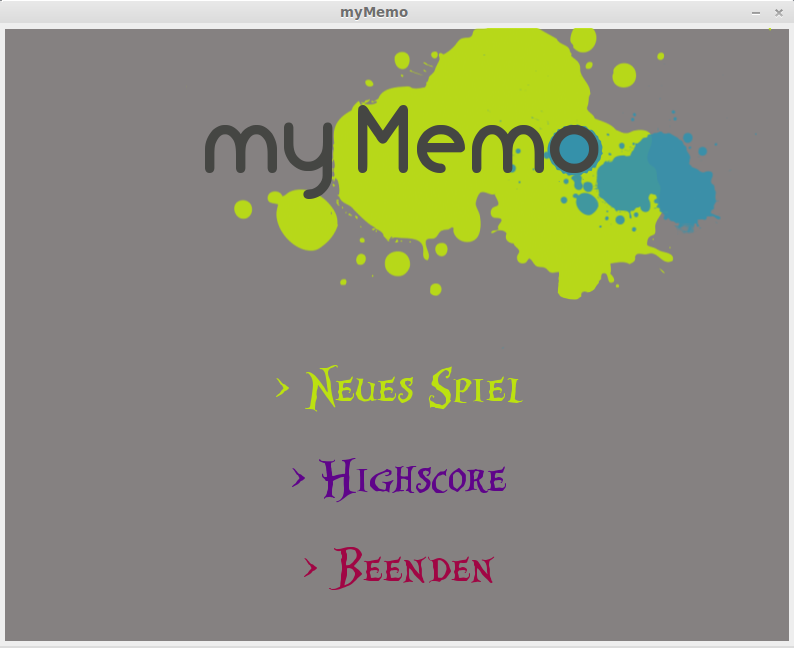
\includegraphics[width=\textwidth]{./guiHauptmenue.png}
	\label{}
\end{figure}
\paragraph{Beschreibung: } Im Hauptmenue kann der Benutzer zwischen den Optionen ,,Neues Spiel``, ,,Highscore`` und ,,Beenden`` wählen. Die Option ,,Neues Spiel`` öffnet Eingabemasken zur Erfassung des Namens und weiterer Wahlmöglichkeiten. Ein Click auf ,,Highscore`` zeigt die aktuelle Highscore an. Der Button Beenden schließt die Anwendung.  


\clearpage
\subsection{Neues Spiel - Spielmodus wählen}
\begin{figure}[!h]
	\centering
    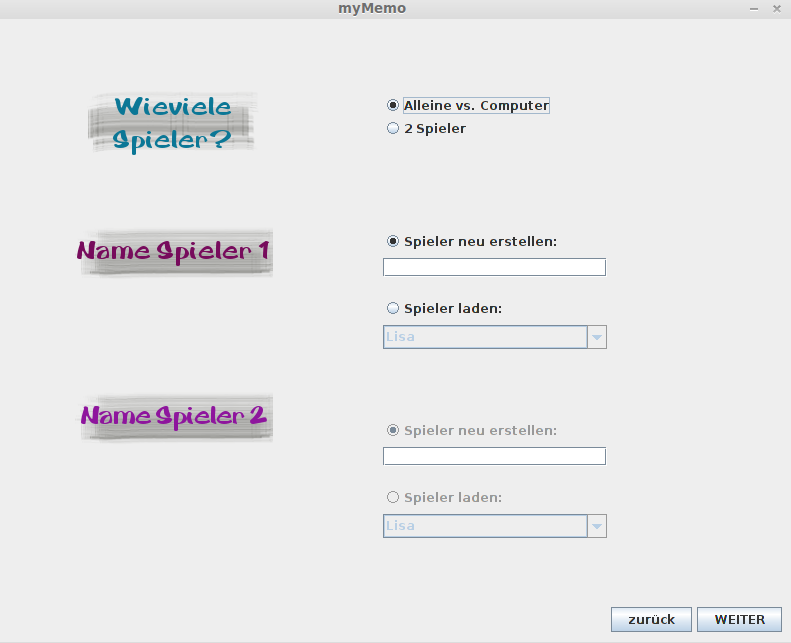
\includegraphics[width=\textwidth]{./guiSpieler.png}
	\label{}
\end{figure}
\paragraph{Beschreibung: }Wurde ,,Neues Spiel'' gewählt, erscheint die obige Maske. In diesem Fall wurde der Spielmodus ,,Alleine vs. Computer'' gewählt. Die Auswahl schaltet die Eingabefelder für den Namen von Spieler 1 frei. Die Eingabefelder von Spieler 2 werden nicht benötigt und sind deshalb nicht editierbar. Der Button ,,zurück'' würde den Benutzer zum Hauptmenue leiten, der Button ,,WEITER'' zur nächsten Eingabemaske für Thema und Spielfeldgröße.

\clearpage
\subsection{Neues Spiel - Spieler erstellen}
\begin{figure}[!h]
	\centering
    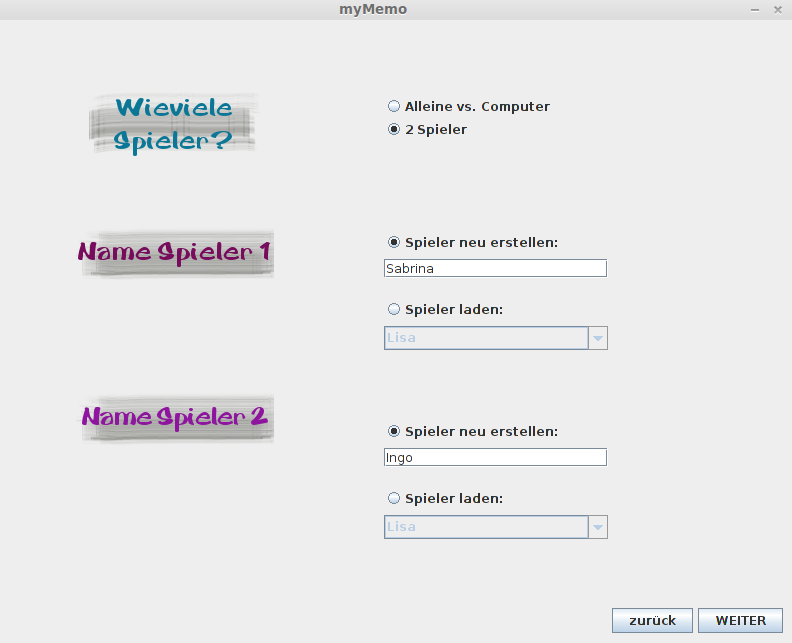
\includegraphics[width=\textwidth]{./guiSpielerNeu.png}
	\label{}
\end{figure}
\paragraph{Beschreibung: }Es wurde der 2-Spieler-Modus gewählt. Nun sind die Eingabefelder für Name von Spieler 1 und Spieler 2 aktiv. Hier wurde in beiden Fällen ein neuer Name erfasst.


\clearpage
\subsection{Neues Spiel - Spieler aus Liste wählen}
\begin{figure}[!h]
	\centering
    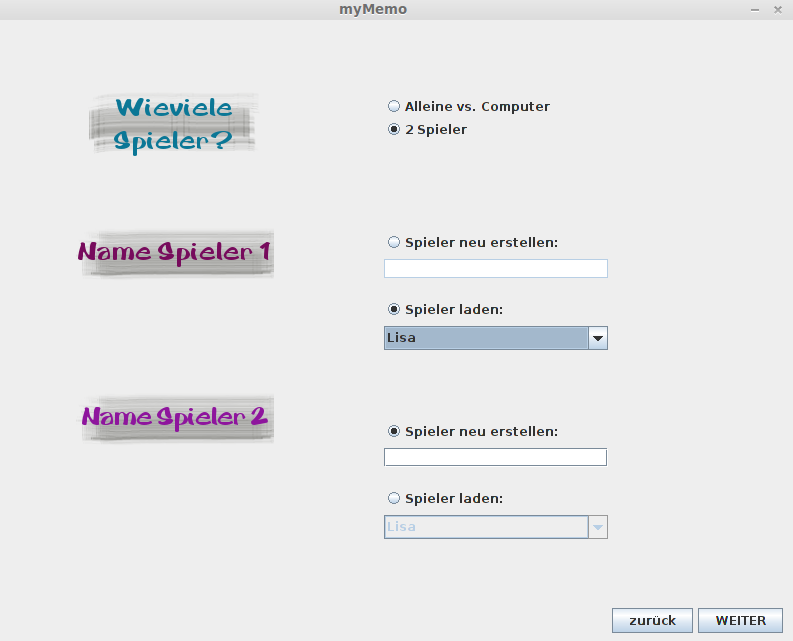
\includegraphics[width=\textwidth]{./guiSpielerListe.png}
	\label{}
\end{figure}
\paragraph{Beschreibung: }Durch den Klick auf den Radiobutton ,,Spieler laden'' wird eine Liste als Dropdown-Menue bereitgestellt. Aus dieser können gespeicherte Namen gewählt werden.


\clearpage
\subsection{Neues Spiel - Prüfung auf doppelten Namen}
\begin{figure}[!h]
	\centering
    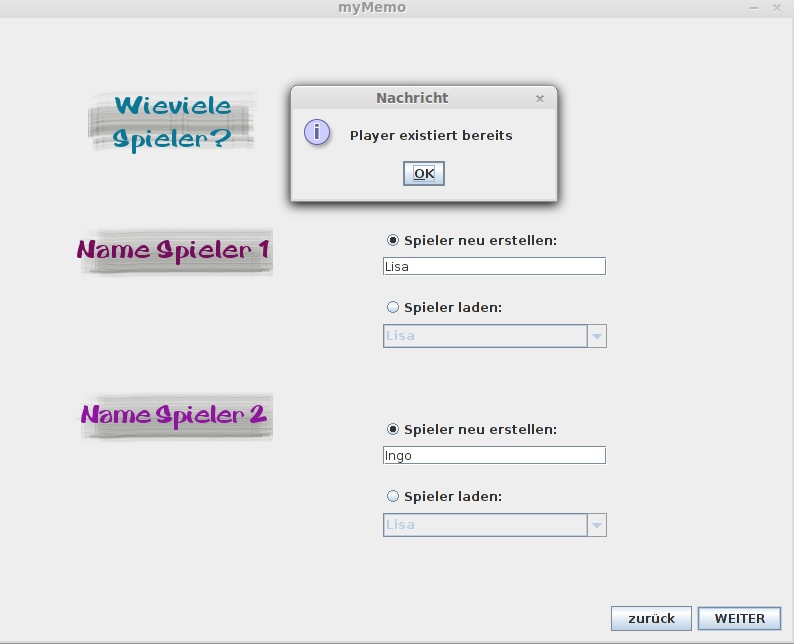
\includegraphics[width=\textwidth]{./guiSpielerError.png}
	\label{}
\end{figure}
\paragraph{Beschreibung: }Bei der Eingabe eines Namens zur Erstellung eines neuen Spielers prüft das System, ob der Name bereits existiert und gibt eine Fehlermeldung aus. Erst nach Änderung und erneuter Prüfung wird durch den Klick auf ,,WEITER'' die nächste Maske aufgerufen.

\clearpage
\subsection{Neues Spiel - Thema und Spielfeldgröße}
\begin{figure}[!h]
	\centering
    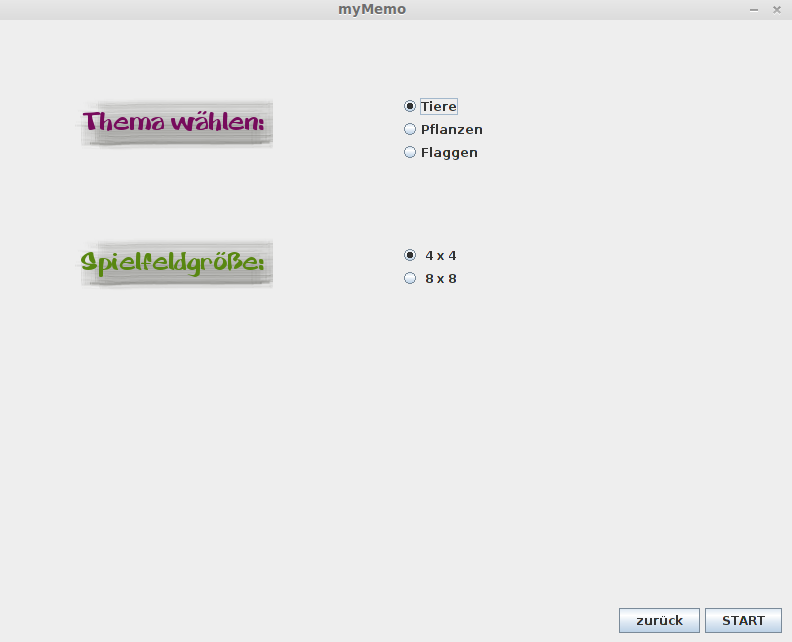
\includegraphics[width=\textwidth]{./guiTiere.png}
	\label{}
\end{figure}
\paragraph{Beschreibung: }Nach Wahl des Spielmodus und Eingabe oder Auswahl des Namens erscheint obige Maske. Hier kann zwischen den Karenthemen Tiere, Pflanzen und Flaggen gewählt werden. Bei der Spielfeldgröße gibt es die Option 4x4 oder 8x8 Karten. Der Klick auf den Button ,,START'' startet das Spiel.


\clearpage
\subsection{Spielfeld}
\begin{figure}[!h]
	\centering
    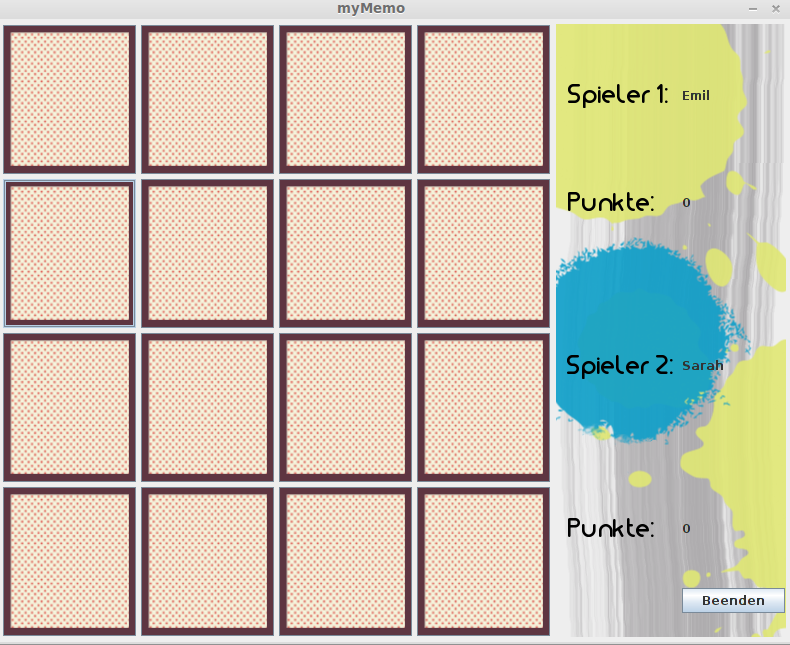
\includegraphics[width=\textwidth]{./guiSpielfeld.png}
	\label{}
\end{figure}
\paragraph{Beschreibung: }Links: Spielfeld mit gemischten Karten und ausgewählten Kartenmotiven. Rechts: Anzeige der Spielerdaten. Es werden die Namen der Spieler und die aktuellen Punkte angezeigt.


\clearpage
\subsection{Spielfeld - Karten gewählt}
\begin{figure}[!h]
	\centering
    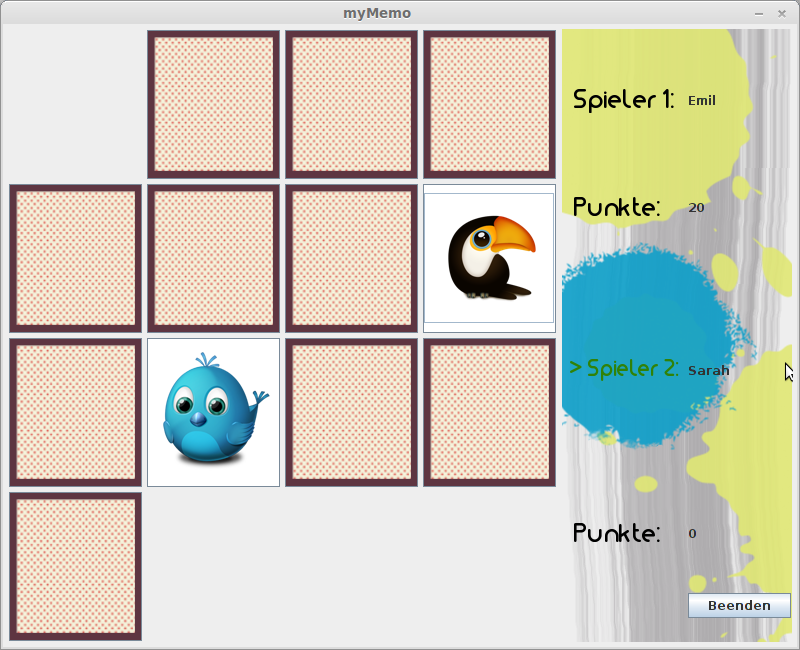
\includegraphics[width=\textwidth]{./guiSpielCards.png}
	\label{}
\end{figure}
\paragraph{Beschreibung: }In dieser Spielsituation hat der Spieler Emil bereits zwei übereinstimmende Kartenpaare gewonnen und somit 20 Punkte erspielt. Jetzt ist Sarah an der Reihe, was durch die farbige Markierung von ,,Spieler 2'' zu erkennen ist. Es sind zwei Karten vom Kartenthema Tiere aufgedeckt.


\clearpage
\subsection{Spielende - Anzeige Gewinnner}
\begin{figure}[!h]
	\centering
    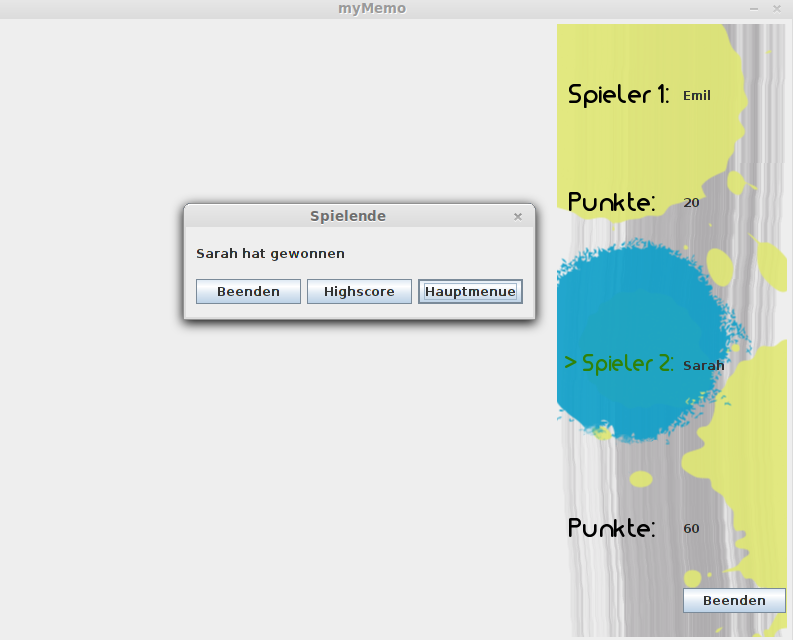
\includegraphics[width=\textwidth]{./guiSpielende.png}
	\label{}
\end{figure}
\paragraph{Beschreibung: }Am Ende des Spiels d.h. wenn alle übereinstimmenden Kartenpaare gefunden wurden, erscheint ein Meldedialog, der den Gewinner mitteilt. Hier hat Sarah mit 60 Punkten gewonnen.


\clearpage
\subsection{Highscore anzeigen}
\begin{figure}[!h]
	\centering
    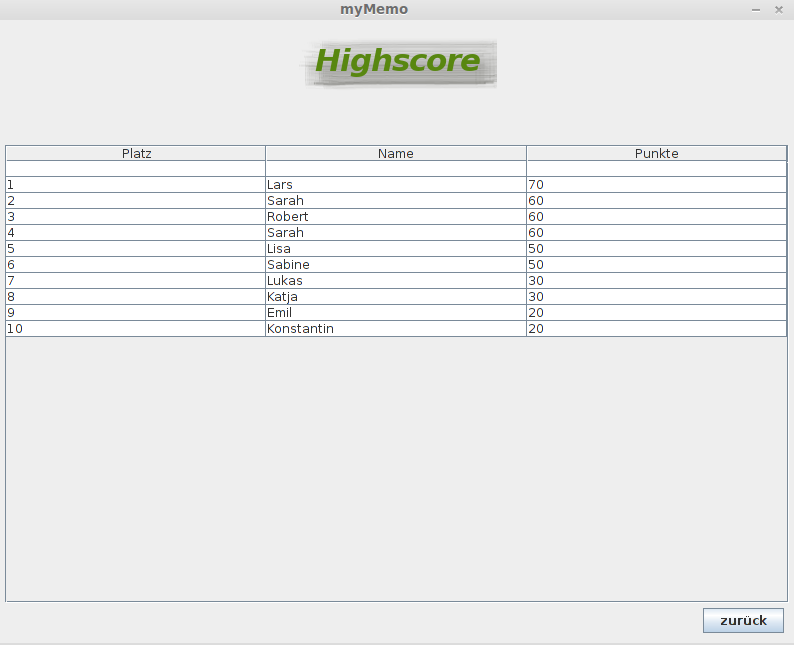
\includegraphics[width=\textwidth]{./guiHighscore.png}
	\label{}
\end{figure}
\paragraph{Beschreibung: } Anzeige der Highscore. Die 10 besten Spieler werden mit ihren erreichten Punkten in Form einer Tabelle aufgelistet.

